
\section{Model architecture} % -------------------------------------
\begin{figure}[htb!]
    \centering
    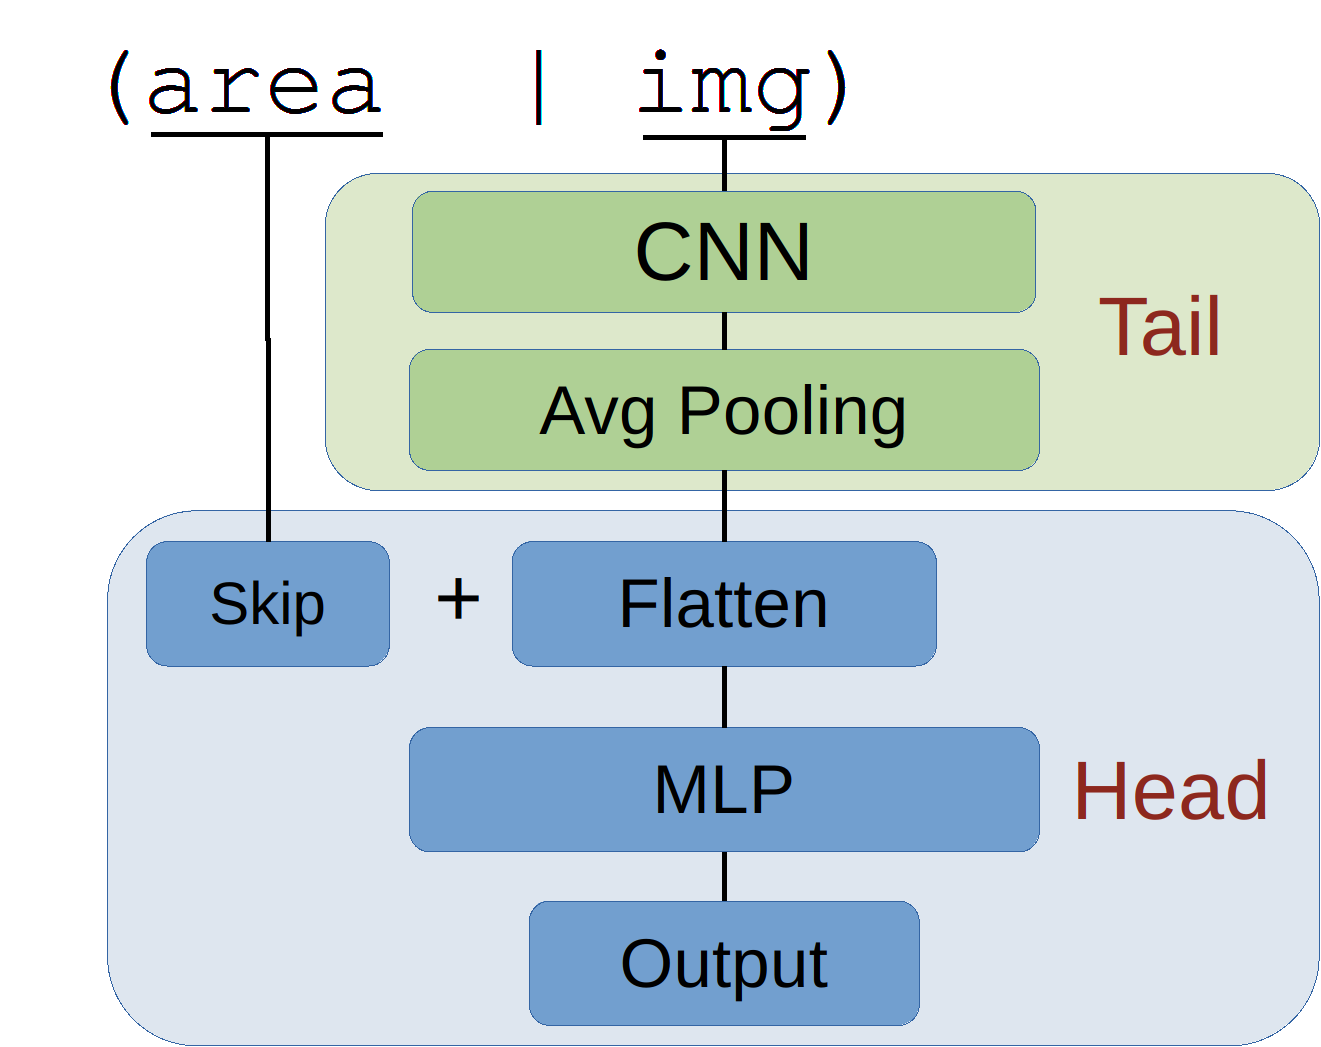
\includegraphics[width=0.55\linewidth]{images/cnnStruct.png}
    \caption{High level overview of the model structure.}
    \label{fig:cnn_arch}
\end{figure}

\noindent
The model can be divided in two distinct sections: a \textit{tail} CNN, responsible for feature extraction, and a \textit{head}, which is a multilayer perceptron (MLP), that produces the output, as shown in \textbf{Figure \ref{fig:cnn_arch}}. 

The fact that the \texttt{area} input is connected to the MLP is due to the image scaling step described in \textbf{Section \ref{sec:dataset_creation}}: the original floorplans are represented in a specific resolution, for which it is known exactly how many pixels in the image represent a meter in the real building, but after rescaling the image to a fixed resolution this information is lost. \\
A robot exploring two environments of different sizes but identical layouts would yield different localization errors, while the model would produce the same output since the scaled input images are identical. Intuitively, an average localization error of $1m$ assumes a radically different meaning if an environment is very small (worse case) or very big. \\
Thus, the skip connection for the area parameter, which in practice becomes a bias term, is needed to compensate for the lost information about the environment size. \\

\noindent
Moreover, in this work we test and compare the performance of three different tail architectures: ResNet \cite{resnet2016}, EfficientNetV2 \cite{efficientnet} and MobileNetV3 \cite{mobileNetV3_2019}. Considering that a hypothetical deployment of this model to a robotic platform would incur in several hardware limitations, by repeating the experiments on these architectures it is possible to empirically assess the performance/inference time trade-off of using one architecture over the other with respect to this specific task. 

% -----------------------------------------------------------
%                                                           \
%                                                           \
% -----------------------------------------------------------

\subsection{Residual networks} % ----------------------------------------------

\begin{figure}[ht!]
    \centering
    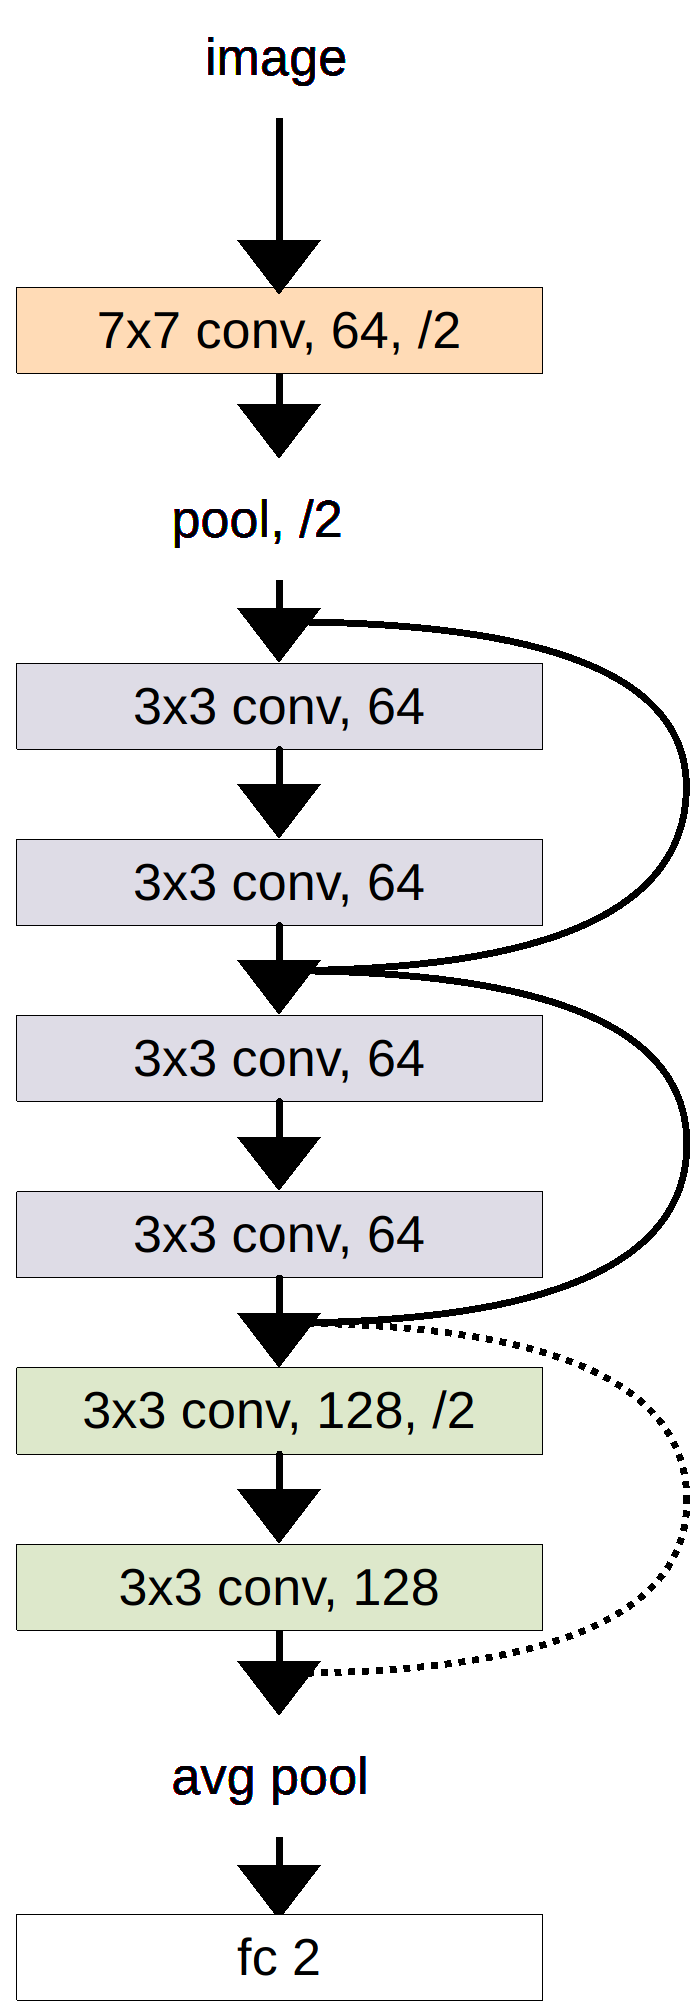
\includegraphics[height=0.8\linewidth, angle=90]{images/convLayers.png}
    \caption{Layer configuration of the custom ResNet.}
    \label{fig:resnet_layers}
\end{figure}
\noindent
The ResNet network has been implemented from scratch, and its layers are summarized in \textbf{Figure \ref{fig:resnet_layers}}. The main characteristic of this architecture is the usage of shortcut connections, represented by the curved lines, which propagates the input matrix of two (or more) stacked blocks and sums it elment-wise to their output (before the activation function). In case the first stacked block reduces the size of its input, the shortcut adjusts the matrix size by performing 1x1 convolutions with a stride of 2 (the dashed shortcut).
These skip connections mitigate the training accuracy degradation phenomenon, where deeper networks converge to a training error higher than shallower ones, indicating that, as the depth of a CNN increases over a certain threshold, the optimizers are not capable of finding better solutions (i.e., it becomes easier getting stuck in a local minima).\\

\noindent
The stacked blocks (i.e., the colored tiles in \textbf{Figure \ref{fig:resnet_layers}}) consist of the following layers:
\begin{itemize}
    \item \textbf{Convolutional layer}, which learns a set of filters (64, 128, or 256) using kernels of size 3x3, except from the first stacked block, which uses a 7x7 kernel. In order to reduce the size of the input tensors, some layers use a stride of two (i.e., the `$/2$' field in the blocks).
    
    \item \textbf{Batch Normalization} \cite{ioffe2015batch}, which normalizes the output of the convolutional layer in order to have zero mean and unit variance, and then applies an additional translation and scaling using two learned parameters $\gamma$ and $\beta$:
    \begin{equation*}
    \begin{split}
        \centering
            &\hat x_i = \frac{x_i - \mu_\mathcal{B}}{\sqrt{\sigma^2_\mathcal{B} + \epsilon}}\\
            &y_i = \gamma\hat x_i + \beta\\
    \end{split}
    \end{equation*}
    Where $x_i$ is the output of the convolutional layer, $\mu_\mathcal{B}$ and $\sigma^2_\mathcal{B}$ are the sample mean and sample variance of the elements of mini-batch $\mathcal{B}$, and $\epsilon$ is an arbitrarily small constant needed for numerical stability.
    
    \item \textbf{Activation layer}: which simply computes the non-linear activation function over the output of the previous layers, in this instance the \textit{ReLU} function: $y_i = max(0, x_i)$. 
\end{itemize}

\noindent
Additionally, the max pooling layer used before the residual blocks, down-samples the feature maps of the preceding convolutional layer; it does so by taking the maximum activation value in a 2x2 kernel passed over each feature map with a stride of two, whereas the average pooling layers takes the average of the activation values in the kernel.\\

\noindent
The EfficientNet and MobileNet architectures are based on residual networks and explore different layer combinations and scaling techniques aimed at reducing inference time and number of parameters, while improving the accuracy of the network.
The EfficientNet and MobileNet weights are pre-trained on the \textit{imagenet} dataset \cite{deng2009imagenet} and are kept frozen; thus, only the MLP weights are adjusted during training.

Instead, the ResNet weights are trained from scratch on our dataset, in order to compare its performance versus that of a CNN trained on a generic classification task (i.e., on \textit{imagenet}). Training a CNN from scratch is a data-hungry process, depending on the network size, but given that the maps used in this work are visually simple and relatively noise-free, a shallow CNN is probably capable of extracting the features needed for our task. Thus, even with a small training set of around 4000 images, it should still be feasible to train a network capable of competing with more complex architectures.


\noindent
Finally, the hidden layers of the MLP, as well as the output layer, use ReLU as the activation function, and the choice on using any regularization technique, such as Batch Normalization or Dropout, is delegated to the hyperparameter selection phase.
